\scanpage{97}
% archive foliation: 99
expliciter le lien du paramètre $a$ avec le paramètre $\tau$, ou
mieux, avec l'invariant modulaire $j\in\mathbb R^{\unsure{2|*}}$ (serait-ce
$j=\unsure{\tfrac14|4}\log a$ ?)
\deleted{\inserted{\unsure{i.e.} $a=\exp j$ ou $a=\exp(-j)$}\unsure{suivant qu'on est dans la famille} $E_a,E'_a$ ?}.

\deleted{Considérons} Notons que si $\sigma$ est dans $G^-$, alors
suivant les cas $-\sigma$ est conjugué, ou non conjugué,
à $\sigma$. \inserted{(réflexion p.r. à la \unsure{droite orthogonale} à celle de $\sigma$)}
Dans le cas hexagonal, il est non conjugué ;
dans le cas carré, il est conjugué. Dans le cas
non \unsure{anharmonique}, $n=2$, il est bien sûr non conjugué (car
$G$ est alors commutatif) -- donc le cas \deleted{hexagonal}\inserted{carré} est
le seul où $-\sigma$ \deleted{\unsure{ne}} soit \deleted{\unsure{pas}} conjugué à $\sigma$.
\deleted{Donc \unsure{si} dans le cas carré par ex., on trouve}
\figure{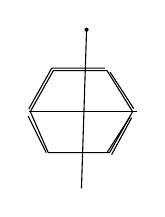
\begin{tikzpicture}[scale=.65]
\draw(-1,0)--(-.55,.8)--(.5,.8)--(1,0)--(.55,-.8)--(-.65,-.8)--cycle;
\draw(-1.03,.05)--(-.58,.85)--(.46,.85);\draw(.56,.77)--(1.02,.06);\draw(-1.04,-.09)--(-.69,-.8);\draw(.95,-.1)--(.5,-.8);\draw(.98,-.12)--(.59,-.84);
\draw(-1.03,0)--(1.08,0);\draw(0,-1.5)--(.1,1.6);\fill(.1,1.6)circle(.04);
\end{tikzpicture}}

\uline{Distinguons les cas}

1) \uline{$n=2$} Cas non \unsure{anharmonique}. Le groupe des autos
est $\pm1,\pm\sigma$, où $\sigma$ est un \inserted{anti} auto. On voit de
suite que si $\sigma$ est du type somme directe d'un
$\operatorname{id}_P$ et $-\operatorname{id}_Q$, il en est de $=$ de $-\sigma$ (avec $P,Q$
échangés) donc on est dans cas $E_a$, \unsure{où}\deleted{\unsure{on}} donc
un $E_a$ et un $E_{a'}$, correspondent aux deux éléments de
$\unsure{\sigma},\sigma'$ de $G^-$, et on aura $aa'=1$.
\deleted{\unsure{En}} car
prenant un gén. $u=\unsure{e_+}$ de $\pi_+$, un autre \inserted{$v=e_-$}$v$ de $\pi_-$, on a
\[
a=a(\sigma)=\frac{Q(\unsure{e_-|e_+})}{Q(e_+)}
\]
et comme par passage de $\sigma$ à $-\sigma$ \deleted{\unsure{les}} $e_+$ et $e_-$ s'interchangent,
on aura bien
\[
a(-\sigma)=1/a(\sigma)
\]
\margin{\figure{\begin{tikzpicture}\draw (0,0)--(0,1.5);\end{tikzpicture}}Ceci vaut aussi bien dans le cas des $E_a$, que des $E'_a$}
(valable dans tous les cas), donc
\[
a(-\sigma)=a(\sigma)\quad\Longleftrightarrow\quad a(\sigma)=1\quad\Longleftrightarrow\quad\text{cas \uline{carré}}.
\]
